\documentclass{subfiles}
\begin{document}
    \begin{figure}[!hb]
        \centering
        \begin{subfigure}{.45\textwidth}
            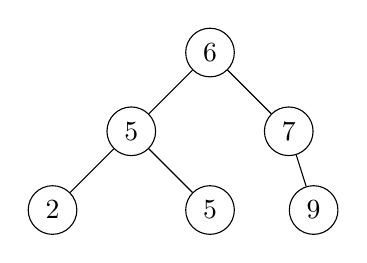
\begin{tikzpicture}
            [
                level distance = 1cm, 
                sibling distance = 2cm,
                every node/.style={
                    draw,
                    circle,
                    minimum size = 0.5cm
                },
            ]

                \node { 6 }
                    child { node {5}
                        child {node {2}}
                        child {node {5}}
                    }
                    child {node {7}
                        child {node [right] {9}}
                    };
            \end{tikzpicture}    
            \caption{}
            \label{Fig:2.a} 
        \end{subfigure}
        \begin{subfigure}{.45\textwidth}
            \begin{tikzpicture}
                [
                ]
                % TODO
            \end{tikzpicture} 
            \caption{}
            \label{Fig:2.b} 
        \end{subfigure}
        \caption{A simple binary tree, alongside its search tree representation.}
    \end{figure}
\end{document}
